\documentclass{beamer}
\usepackage{amsmath}
\usepackage{tikz}
\usepackage{amsmath}
\usepackage{tikz-cd}


% Presentation information
\title{Mathematics is just more language}
\author{Hans Halvorson}
\date{December 6th}

\usetheme{metropolis}

%% possibly something about "intrinsic" formulations. Think about the
%% Sider thing about theories stating relations between physical
%% objects and numbers 

\begin{document}

% Title slide
\begin{frame}
    \titlepage
\end{frame}

\section{Overview} 

\begin{frame}

  \begin{itemize}
  \item Mathematics is hybrid: it is both an object of thought and a
    tool of thought.
  \item Late 20th century analytic philosophy focused almost
    exclusively on mathematics as ``object of thought'', i.e.\
    something we have theories \emph{about}.
  \item If mathematical stuff is just additional stuff to think
    \emph{about}, then Ockhamist considerations would suggest trying
    to do without it.
  \item If we are thinking \emph{with} mathematics, then it is no more
    dispensable than concepts or language. \end{itemize}


  \end{frame}

\section{A narrative}

\begin{frame}{History of the philosophy of applied mathematics}

  \begin{itemize}
  \item Pre 19th century, through Kant \newline I imagine that it
    didn't occur to anyone that commitment to mathematical theories
    was optional.
  \item Non-euclidean geometries
  \item Conventionalism
  \end{itemize}

\end{frame}

\begin{frame}{History of the philosophy of applied mathematics}

  \begin{itemize}
  \item Carnap's frameworks
  \item Quine's package deal
  \item Field's program 
  \end{itemize}

\end{frame}

\begin{frame}{History of the philosophy of applied mathematics}

  \begin{itemize}
  \item HH: The absurdity to which Field's program leads uncovers
    something deeply wrong at the heart of Quine's view.
  \item HH: Quine errs in attempting to describe everything from a
    third-person point of view.
  \item But I will leave that here --- it's murky philosophy that we
    can avoid today.
  \end{itemize}

\end{frame}

\begin{frame}

  %% Bohr quote

  ``Mathematics is not to be regarded as a special branch of knowledge
  based on the accumulation of experience but rather as a
  \textbf{refinement of general language}, supplementing it with
  appropriate tools to represent relations for which ordinary verbal
  expression is imprecise or too cumbersome.'' (Niels Bohr)


\end{frame}

\section{Field's program}

\begin{frame}{The Putnam-Quine indispensability argument}

  \begin{itemize}
  \item The ideally rational person accepts the best scientific
    theories and all the things that they are committed to. 
  \item (Indispensability) Our best scientific theories cannot
    dispense with mathematical objects.
  \item The ideally rational person is a mathematical Platonist.
  \end{itemize}

\end{frame}

\begin{frame}{Two responses}

  \begin{itemize}
  \item Fictionalism: Reject the first premise, you don't have to take
    all those things literally.
  \item Eliminativism: Reject the second premise by showing that our
    best scientific theories can dispense with mathematical
    objects. \newline Hartry Field: Replace the Platonistic $T$ with a
    nominalistic version $N(T)$. 
  \end{itemize}

\end{frame}

\begin{frame}

  ``If they do not exist, should not it be possible, at least in
  principle, to characterize the physical world without talking about
  them at all? Here is another job for philosophers: to find
  alternatives to standard `platonistic'
  (mathematical-entity-invoking) physical theories which can do the
  same empirical explanatory work without requiring any mathematical
  entities to exist.'' (Arntzenius and Dorr, 2012)

\end{frame}

\begin{frame}{Motivating example}

  Field takes the relationship between numerical and synthetic
  geometry as a paradigm example of nominalization.

  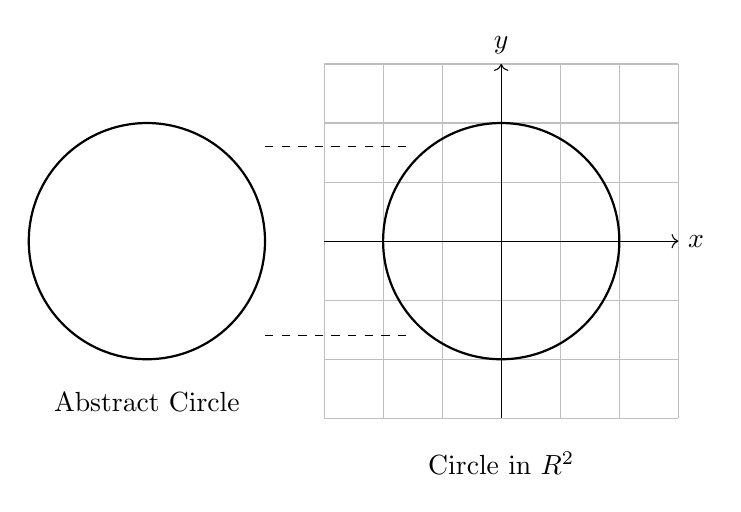
\begin{tikzpicture}[scale=1.5]

% Circle on the left (abstract, no coordinate axes)
\draw[thick] (-3,0) circle (1);
\node[below] at (-3,-1.2) {Abstract Circle};

% Cartesian coordinate system on the right with grid
\draw[step=0.5,gray!50,thin] (-1.5,-1.5) grid (1.5,1.5); % Light gray grid
\draw[->] (0,-1.5) -- (0,1.5) node[above] {$y$};
\draw[->] (-1.5,0) -- (1.5,0) node[right] {$x$};
\draw[thick] (0,0) circle (1);
\node[below] at (0,-1.7) {Circle in $\mathbb{R}^2$};

% Dashed lines linking the circles
\draw[dashed] (-2,0.8) -- (-0.8,0.8);
\draw[dashed] (-2,-0.8) -- (-0.8,-0.8);

\end{tikzpicture}

\end{frame}

\section{Worries about Field's program}

\begin{frame}{Nominalizing by fiat}

  \begin{itemize}
  \item For any theory $T$, interpret all terms as applying to some
    kind of ``physical'' stuff.
  \item Arntzenius: We use fiber bundles in physics, so let us assume
    that elements of a fiber bundle are real physical things.
  \item Schroeren: We use symmetry groups in physics, so let us assume
    that the group elements are real physical things.
  \end{itemize}

\end{frame}

\begin{frame}

  ``The mathematics of phase space is part of the genuine content of
  classical mechanics. This bit of the mathematics used in our physics
  cannot be representationally inert: it is inherent to the
  dynamics. One way to spell this out further would be to be a
  substantivalist about statespace. Again, I happen to be open to the
  idea. But we need not go that way. The important thing is that phase
  space is not just a mathematical convenience. Some part of reality
  is more or less directly represented by it.'' (North 2009)

\end{frame}


\begin{frame}{Nominalizing by fiat}

  \begin{itemize}
  \item Field takes $\mathbf{RCF}$ to be quantifying over numbers, but
    $\mathbf{E}^2$ to be quantifying over physical objects.
  \item I'm not interested in non-mathematical properties of theories.
  \end{itemize}
  
\end{frame}


\begin{frame}{Ontological commitment is overrated}

  \begin{itemize}
  \item Autobiography: I wasn't committing to Platonism when I used a
    vector space to describe the sum of two forces.
  \item A Morita extension of $T$ adds new domains of quantification.
  \item Morita equivalent theories need not agree on how many things
    there are.
  \item What's an object and what's vocabulary can depend on
    formulation.
  \end{itemize}
  
\end{frame}




\begin{frame}{Concrete mathematics is closer to reality}

  \begin{itemize}
  \item Claim: Field has it backwards in thinking that synthetic
    geometry is closer to \emph{Anschauung} than numerical geometry.
  \item Syntactically: Assigning physical extensions to terms in the
    signature of $Th(\mathbb{R}^2)$ is \emph{easier} than assigning
    physical extensions to terms in the signature of $\mathbb{E}^2$.
  \item Syntactically: Assigning elements of $\mathbb{R}^2$ to points
    of space is \emph{easier} than assigning elements of a model $M$
    of $\mathbb{E}^2$.
  \end{itemize}

\end{frame}

\begin{frame}{Concrete mathematics is closer to reality}

  \begin{itemize}
  \item A perfect circle is a classic example of a Platonic object
  \item An extensionless point is a classic example of a Platonic
    object
  \end{itemize}

\end{frame}


\begin{frame}{The argument form}

  GTR is the best theory of gravitational phenomena. 

  GTR uses smooth manifolds. 

  Smooth manifolds live in a model of ZF set theory.

  GTR entails the truth of ZF set theory.

  The best theory of gravitational phenomena is committed to the
  existence of sets.

\end{frame}

\begin{frame}{The argument form}

  GTR uses symbols such as ``$g_{ab}$''. 

  The best theory of gravitational phenomena is committed to the
  existence of symbols.

\end{frame}


\begin{frame}{On quantifying over numbers or sets}

  In realistic examples, it is unclear what a mathematical theory
  quantifies over.

  \begin{itemize}
  \item A smooth manifold $M$ has a collection of coordinate charts,
    each of which is a mapping to $\mathbb{R}^n$.
  \item A Hilbert space is a vector space over $\mathbb{C}$.
  \item A $C^*$-algebra is a set $A$ with a function
    $\mathbb{C}\times A\to A$.
  \item The dual of a group $G$ is the set of mappings of $G$ into the
    circle group $\mathbb{T}$.
  \end{itemize}

\end{frame}


\section{A meta-pragmatist manifesto}


\begin{frame}{A meta-pragmatist manifesto}

    \begin{itemize}
    \item I want to know what difference our philosophical ruminations
      and theories might make for scientific practice.
    \item Example: The claim that ``wave mechanics and matrix
      mechanics are equivalent'' should end the search for experiments
      or arguments that would favor one of the two.
    \item Example: If Lagrangian and Hamiltonian mechanics are
      inequivalent, then physicists should change their practice.
    \end{itemize}  

\end{frame}

\begin{frame}

    \begin{itemize}
    \item Claim: Something between Morita equivalence and categorical
      equivalence is the best proposal we have for scientific
      practice.
    \item This claim is not an attempt to describe (as ``naturalists''
      would want), nor is it an attempt to regulate science with
      ariori philosophical insight. Rather, it is
      \textbf{explicative}.
    \end{itemize}

  \end{frame}

\section{Back to Wissenschaftslogik!}  

  \begin{frame}{Carnap's call for objectivity}

  
\includegraphics[scale=0.4]{~/talks/formal.jpg}


\end{frame}

\begin{frame}{Non-mathematical properties of theories}

  \begin{itemize} 
  \item Neil Dewar is thinking about $T$
  \item $T$ is about birds  
  \item $T$ is nominalistic
  \item $T$ quantifies over mathematical objects
  \end{itemize}

\end{frame}



\begin{frame}{Mathematical properties of theories}

  \begin{itemize}
  \item $T$ is finitely axiomatizable  
  \item $T$ is $\aleph _0$-categorical
  \item There is a conservative translation $F:T\to T'$
  \end{itemize}

\end{frame}

\begin{frame}{Mathematical properties of theories}

  \begin{itemize}
  \item We are most interested in properties that are invariant under
    the relevant notion of theoretical equivalence.
  \item For example, ``$T$ has the symbol `$P$' in its signature'' is
    not invariant.
  \end{itemize}

\end{frame}

\begin{frame}{Three perspectives on theories}

  \begin{itemize}
  \item Syntax
    \begin{itemize}
    \item Objects: A set of axioms in a formal language
    \item Arrows: $n$-dimensional interpretations
    \end{itemize}  
  \item Semantics
    \begin{itemize}
    \item Objects: A category of models with some (elusive!)
      additional structure
    \item Arrows: Functors that preserve the additional structure
    \end{itemize}
  \end{itemize}

\end{frame}  

\begin{frame}{Three perspectives on theories}

    \begin{itemize}
    \item Hybrid
      \begin{itemize}
      \item Objects: Syntactic categories, e.g.\ coherent categories
      \item Arrows: coherent functors
      \end{itemize}
    \end{itemize}
      
\end{frame}


\section{The 2-category of first-order theories}



\begin{frame}[fragile]{The 2-category of first-order theories}

\[
\begin{tikzcd}[row sep=2.5em, column sep=4em]
T \arrow[bend left=50]{r}[name=U]{F} \arrow[bend right=50]{r}[name=D,
below]{G} & T' \arrow[Rightarrow, from=U, to=D, shorten >=3pt, shorten <=3pt]
\end{tikzcd}
\]


\end{frame}

\begin{frame}{The 2-category of first-order theories}

  \begin{itemize}
  \item Definition: $F:T\to T'$ is conservative if $T'\vdash F\phi$
    implies $T\vdash \phi$.
  \item Definition: $F:T\to T'$ is essentially surjective if for each
    $\psi\in \Sigma '$, there is a $\phi\in \Sigma$ such that
    $T'\vdash \psi \leftrightarrow F\phi$.
  \item How to define essentially surjective for $n$-dimensional
    translations?
  \end{itemize}

\end{frame}



\section{Revamping Field's program}

\begin{frame}

  \begin{itemize}
  \item Field: The desired result is that $T$ is a
    \textbf{conservative extension} of $N(T)$.
  \item Analogy? $T=N(T)+\{ c\}$
  \item HH: No, there is a more interesting relationship where $T$ is
    like a covering space of $N(T)$
  \item Analogy? The relationship of an affine space to its underlying
    vector space
  \end{itemize}

\end{frame}

\begin{frame}

  \begin{itemize}
  \item Intuitively, there is a model of $\mathbf{E}^2$ in
    $\mathbb{R}^2$.
  \item There is a translation of $\mathbf{E}^2$ into $\mathbf{RCF}$.
  \item Zayton: There is a more interesting relationship between
    $\mathbf{RCF}$ and $\mathbf{E}^2$ having to do with
    interpretations with parameters.
  \end{itemize}

\end{frame}

\begin{frame}

  \begin{itemize}
  \item Field was probably thinking of the Platonist theory as a
    theory $T'$ with two sorts, physical objects and numbers, and with
    a function $f$ from objects to numbers.
  \item But $T'$ is Morita equivalent to $Th(\mathbb{R}^2)$.
   \end{itemize}    

 \end{frame}

 \section{Conclusion}

 % Closing slide
\begin{frame}{Conclusion}

  \begin{itemize}
  \item What attitude should we take toward mathematical language that
    is employed in empirical science?
  \item I find the question to be too abstract. Compare with: what
    kind of attitude should I take to works of art?
  \item Hartry Field gives a concrete theory-building proposal:
    \textit{replace Platonistic theories by nominalistic theories}.
  \end{itemize}

\end{frame}

\begin{frame}{Conclusion}

  \begin{itemize}
  \item Field's proposal fails Carnap's concreteness test.
  \item What proposals do you have for improving our use of
    mathematical language in science? 
  \end{itemize}
    

\end{frame}  


 \end{document}





    

\begin{frame}

    ``It's fine to construct models with artefacts. But there must
    always be some way of describing the phenomenon in question that
    (in some sense) lacks artefacts. There must be some way of saying
    what is really going on. For example, although we can model mass
    with real numbers, there must be some underlying artefact-free
    description, such as the $\succeq$ and $C$ description, from which
    one can recover a specification of which numerical models are
    acceptable, and a specification of which features of the models
    are artefacts.'' (Ted Sider) 

  \end{frame}


\begin{frame}{A Carnapian approach to theories}

  \begin{itemize}
  \item Key idea: Using a framework, or being situated in a framework,
    differs in important ways from \emph{commitment} to the truth of
    any claims.
  \item Example: If I learn a new language, I am not \emph{eo ipso}
    adopting any new beliefs.
  \item I recommend against taking ``framework'' to be a natural kind.
  \end{itemize}

\end{frame}


\begin{frame}{A Carnapian approach to theories}

  \begin{itemize}
  \item Quine: I don't understand the difference between adopting a
    framework and committing to the claims of the framework.
  \item HH: Of course you can't, because you don't have a robust
    notion of \emph{belief} qua mental state.
  \end{itemize}



\end{frame}

\begin{frame}{Objectivizing theories}

  \begin{itemize}
  \item Michael Friedman: Quine et al. missed the fact that the
    positivists were concerned with objectivity.
  \item HH: Quine et al. missed the fact that the positivists were
    concerned with practical guidance.
    \begin{itemize}
    \item If one wants to do work on a theory, there should be
      objective benchmarks for what improvement would look like.
    \end{itemize}
  \end{itemize}

\end{frame}



\begin{frame}{Carnap was on the right track}

  \begin{itemize}
  \item The important distinction isn't between syntax and semantics,
    it's between mathematical and non-mathematical.
  \item In this broader sense of ``mathematical'', there are powerful
    tools for modelling relations between theories.
  \end{itemize}

\end{frame}

  

% Section 1


\begin{frame}{Carnap's challenge}

  \begin{itemize}
  \item Proposal: A property of a theory, or a relation between
    theories, is objective insofar as it can be defined
    ``syntactically''
  \item Criticism: This requirement is unclear. Is it a syntactic
    property of a theory $T$ that it interprets Peano arithmetic?
  \end{itemize}


\end{frame}




% Section 3

  \begin{frame}

    Semantics and the temptation to Pythagoreanism

    How syntax can help us avoid Pythagoreanism

    Worthy projects: Determining what is definable (e.g. Curiel's work
    on definability in terms of the metric tensor field)



\end{frame}




\end{document}

%%% Local Variables:
%%% mode: latex
%%% TeX-master: t
%%% End:

\begin{frame}{Dethroning Tarskian model theory}

  \begin{itemize}
  \item Democracy of theories --- including ZF set theory.
  \item Interpretation of theories in categories other than the
    category of sets.
    \begin{itemize}
    \item Synthetic differential geometry is classically inconsistent,
      but has interpretations in intuitionist toposes.
    \item A topological group is a group object in the category of
      topological spaces.
    \end{itemize}
  \end{itemize}

\end{frame}

\begin{frame}{Dethroning Tarskian model theory}

\begin{itemize}
  \item Open question: What's the right way to understand a Tarskian
    model of $T$ in terms of translations between $T$ and other
    theories, either the empty theory, or some set theory?
\end{itemize}


\end{frame}



  \begin{frame}

    I don't know if I'm a Platonist or not.

    I don't feel an urge to avoid Platonism at all costs. But I do
    want to understand norms for using mathematics in science.

    The ``hard problem'' for philosophy of mathematics: given that one
    is a realist about physical things, then what is the relationship
    between those things and mathematics?

    The Pythagorean solution: Physical stuff \emph{is} mathematical
    stuff.

  \end{frame}

  \begin{frame}

    Claim 1: Fear of human subjectivity drives philosophers to the
    Pythagorean solution.

    Claim 2: The Pythagorean solution is a kind of insanity.

  \end{frame}

  \begin{frame}

    ``The definition of mathematical symbols and operations is based
    on simple logical use of common language. Mathematics is therefore
    not to be regarded as a special branch of knowledge based on the
    accumulation of experience but rather as a \textbf{refinement of
      general language}, supplementing it with appropriate tools to
    represent relations for which ordinary verbal expression is
    imprecise or too cumbersome.'' (Niels Bohr)


  \end{frame}


  \begin{frame}

    Plato pushes in the direction of the distinct reality of physical
    objects: they merely ``participate'' in the forms

    

    Two different diseases, caused by a common misconception of the
    relationship between mathematics and concrete reality.

    Hartry Field \: Ted Sider \: David Wallace 


  \end{frame}
